\chapter{На каких языках программирования пишутся операционные системы}
\label{ch:operating-sysmets}

В статье исследуется объект Викиданных <<операционная система>> (operating system) и его свойства. В каждом из разделов представлены задачи, решённые с помощью SPARQL-запросов. В их числе: нахождение экземпляров объекта <<операционная система>>, построение списка операционных систем (ОС) по предку, по времени создания, по языку, на котором написана ОС. Также построена гистограмма, показывающая количество программ, написанных на том или ином языке программирования, и долю того, сколько из них работает под той или иной ОС. У многого программного обеспечения не указан язык программирования, на котором оно разрабатывалось. Для улучшения результатов решения вышеописанных задач отдельные объекты Викиданных были дополнены свойством <<язык программирования>>.


\section{Экземпляры объекта <<Операционные системы>>}
Ниже представлен SPARQL-запрос для получения списка всех операционных систем (листинг \ref{lst:all_operating_systems}).

\begin{lstlisting}[ language=SPARQL, 
caption={\href{https://w.wiki/n89}{Список всех опрационных систем}\protect\footnotemark},
label=lst:all_operating_systems, 
escapebegin=ку,escapeend=ку-ку>
]
SELECT ?os ?osLabel
WHERE
{
	?os wdt:P31 wd:Q9135. # instance of operating system
	SERVICE wikibase:label { bd:serviceParam wikibase:language "ru, en" }
}
\end{lstlisting}
\footnotetext{Получено \num{510} операционных систем в 2017 году, и \num{1086} в 2020 году.  Ссылка на SPARQL-запрос: \href{https://w.wiki/n89}{https://w.wiki/n89}}

[+] Наиболее полными и проработанными операционными системами на Викиданных являются: \wdqName{Linux}{388}, \wdqName{Microsoft Windows}{1406}, \wdqName{Windows 8}{5046}

[-] Почти пустыми и малоинформативными операционными системами оказались: \wdqName{SPIN}{16314510}, \wdqName{JavaOS}{1684163}, \wdqName{Atari TOS}{1574899}, \wdqName{Xubuntu}{72688}

По данным ProWD у единственной в Викиданных отечественной операционной системы \wdqName{Miraculix}{4044344} 7 свойств \cite{prowd_os_link}. Лидерами по операционным системам всего мира являются \wdqName{Microsoft Windows}{1406} и \wdqName{Windows 8}{5046} имеющие по 24 свойства.


\section{На чем основаны ОС}
Ниже представлен SPARQL-запрос для получения списка основы операционных систем (листинг \ref{lst:base_of_operating_systems}).


\marginnote{
	Выберите ОС, на основе которой создано больше всего других ОС:
	\begin{itemize}
		\item \href{https://w.wiki/n8U}{Debian}
		\item \href{https://w.wiki/n8V}{Android}
		\item \href{https://w.wiki/n8W}{Ubuntu}
		\item \href{https://w.wiki/n8X}{Linux kernel}
	\end{itemize}
	См. ответ~\ref{answer:what_system_created} на с.~\pageref{answer:what_system_created}.
}

\begin{lstlisting}[ language=SPARQL, 
caption={\href{https://w.wiki/n8F}{Список основ опрационных систем}\protect\footnotemark},
label=lst:base_of_operating_systems, 
escapebegin=ку,escapeend=ку-ку>
]
SELECT ?osLabel ?baseLabel
WHERE
{
	?os wdt:P31 wd:Q9135. # instance of operating system
	?os wdt:P144 ?base. # base on 
	SERVICE wikibase:label { bd:serviceParam wikibase:language "ru, en" }
}
GROUP BY ?osLabel ?baseLabel
\end{lstlisting}
\footnotetext{Получено \num{47} результатов в 2017 году, и \num{118} в 2020 году. Ссылка на SPARQL-запрос: \href{https://w.wiki/n8F}{https://w.wiki/n8F}}

Данный запрос показывает соответствие между <<Операционной Системой>> и ее <<предком>>, на котором она основана.


\section{Время выпуска ОС}
\marginnote{
	Какую из этих операционных систем разработала компания \href{https://w.wiki/n8S}{Apple}?
	\begin{itemize}
		\item \href{https://w.wiki/n8P}{Newton OS}
		\item \href{https://w.wiki/n8Q}{Ubuntu Touch}
		\item \href{https://w.wiki/n8R}{JavaOS}
	\end{itemize}
	См. ответ~\ref{answer:what_system_created} на с.~\pageref{answer:what_system_created}.
}

Ниже представлен SPARQL-запрос для получения списка операционных систем с датой их создания (листинг \ref{lst:inception_time_of_operating_systems}).
\begin{lstlisting}[ language=SPARQL, 
caption={\href{https://w.wiki/n8A}{Список операционных систем с датой их создания}\protect\footnotemark},
label=lst:inception_time_of_operating_systems, 
escapebegin=ку,escapeend=ку-ку>
]
SELECT ?osLabel ?time
WHERE
{
	?os wdt:P31 wd:Q9135. # instance of operating system
	?os wdt:P571 ?time. # inception time
	SERVICE wikibase:label { bd:serviceParam wikibase:language "ru, en" }
}
GROUP BY ?osLabel ?time
ORDER BY DESC(?time)
\end{lstlisting}
\footnotetext{Получено \num{30} результатов в 2017 году, и \num{238} в 2020 году. Ссылка на SPARQL-запрос: \href{https://w.wiki/n8A}{https://w.wiki/n8A}}

Данный запрос показывает в красивой графической оболочке таймлайн создания(на самом деле выпуска) операционных систем. А еще так-же он показывает насколько плохо заполнены викиданные, так как в запросах выводится только 238 результатов. Что в свою очередь обозначает что у других <<объектов>> это поле попросту не заполнено. Хотя информация о <<дате выпуска>> не такая уж и секретная.

\section{Кол-во ОС написанных на языках программирования}
Ниже представлен SPARQL-запрос для получения списка языков программирования с количеством написанных на них ОС (листинг \ref{lst:count_os_on_languages}).

\begin{lstlisting}[ language=SPARQL, 
caption={\href{https://w.wiki/n8B}{Список языков программирования с количеством написанных на них ОС}\protect\footnotemark},
label=lst:count_os_on_languages, 
escapebegin=ку,escapeend=ку-ку>
]
SELECT ?lang (count(*) as ?count)
WHERE 
{
	?os wdt:P31 wd:Q9135. # instance of operating system
	?os wdt:P277 ?langObj. # created on programming language
	OPTIONAL {
		?langObj rdfs:label ?lang
		filter (lang(?lang) = "en")
	}
}
GROUP BY ?lang
ORDER BY DESC(?count) ASC(?lang)
\end{lstlisting}
\footnotetext{Получено \num{24} результатов в 2017 году, и \num{37} в 2020 году. Ссылка на SPARQL-запрос: \href{https://w.wiki/n8B}{https://w.wiki/n8B}}

Данный запрос показывает (только на основе заполненых викиданных, поэтому не факт что это правда) что преимущественно ОС пишут на языке Ассемблер, что несомненно является правдой, потому что это самый быстрый, но при этом удобный язык программирования. На втором и третьем месте разместились Си и C++, которые в свою очередь являются не худшим аналогом, так как несмотря на свою (относительно Ассемблера) <<медленность>>, они наиболее удобные и понятные ЯП.


\section{Полнота данных}
По данным на 2017 год с сайта www.operating-system.org удалось установить что существует порядка 611 операционных систем \cite{list_operating_systems} (не учитывая дистрибутивы Linux'а, коих количество превышает количество самих операционных систем). В то время как викиданные содержат информацию лишь о 510 операционных системах. И если просмотреть достаточно большое количество объектов из запрос, то станет ясно еще и то, что много из них еще и не очень хорошо заполнены, а то и вовсе практически пусты.

В 2020 году викиданные содержат информацию о 1086 операционных системах, что свидетельствует о значительных изменениях, однако большое количество объектов по-прежнему плохо заполнены. Из этого можно сделать вывод о неполноте викиданных.

\section{Языки программирования, используемые для написания операционных система}
Если взглянуть на количество операционных систем, для которых указано свойство <<язык программирования>>, то можно увидеть что из 1086 объектов это свойство заполнено лишь у 116. Но по существующим данным на рис.~\ref{fig:count-os-written-on-languages} можно определить, что большинство операционных систем написаны на языке программирования C. 
\begin{figure*}[h!]
	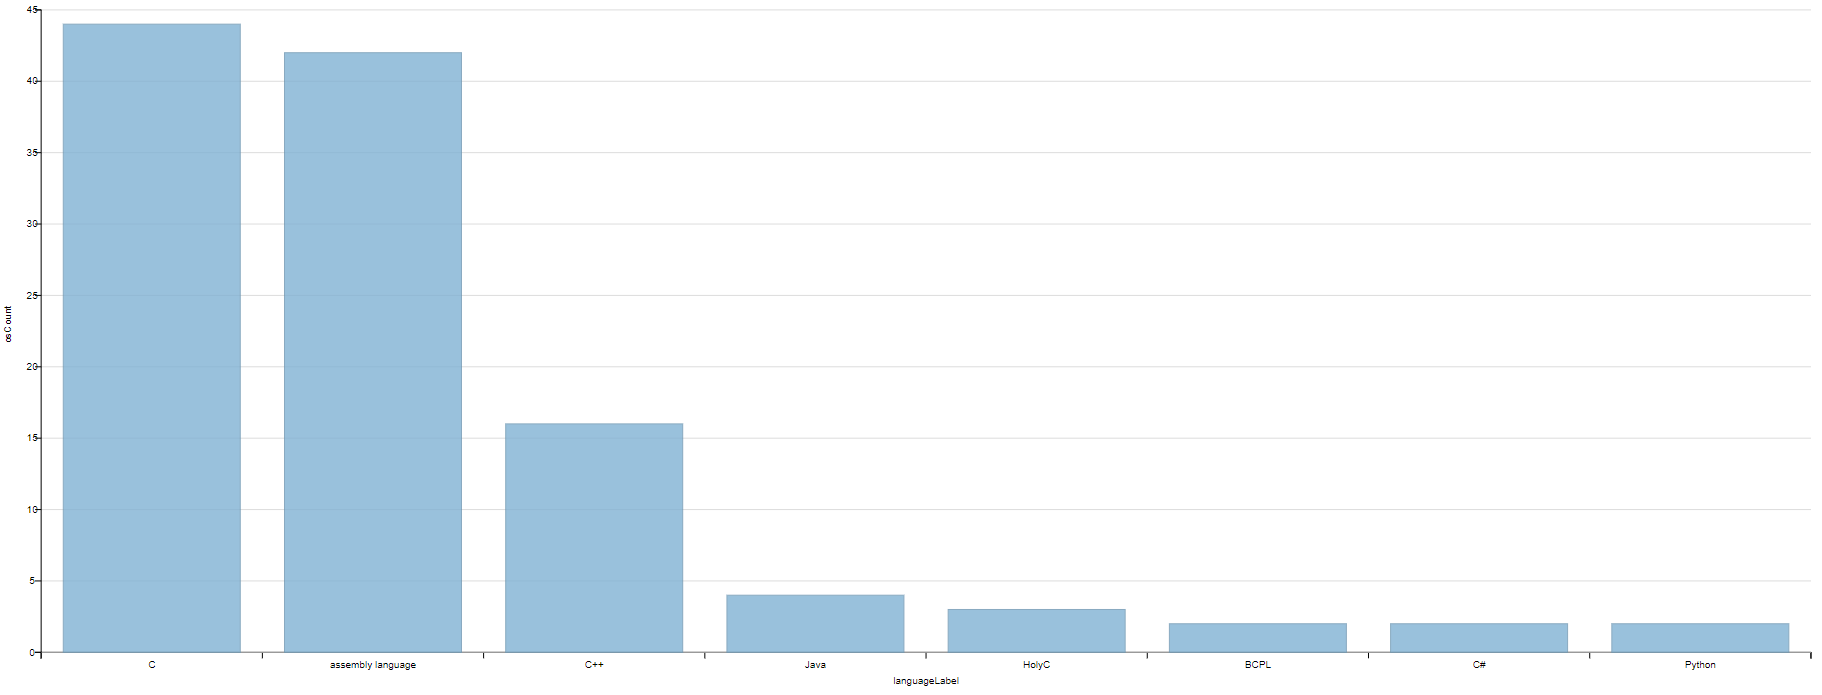
\includegraphics{./chapter/operating_system/count-os-written-on-languages.png}
	\caption{Количество операционных систем, написанных на языках программирования (данные на 2020 год.)}
	\label{fig:count-os-written-on-languages}
\end{figure*}


\section{Запрос показывает для каждого софта под каждую ОС на скольких языках он написан}
Ниже представлен SPARQL-запрос показывающий для каждого софта под каждую ОС на скольких языках он написан (листинг \ref{lst:count_soft_on_os}).

\begin{lstlisting}[ language=SPARQL, 
caption={\href{https://w.wiki/n8C}{Список ос с количеством сфота для него}\protect\footnotemark},
label=lst:count_soft_on_os, 
escapebegin=ку,escapeend=ку-ку>
]
SELECT ?soft ?softLabel ?os ?osLabel (count(*) as ?count)
WHERE
{
	?soft wdt:P306 ?os. # operating system on which a software works
	?soft wdt:P277 ?lang. # programming language in which soft is developed
	SERVICE wikibase:label { bd:serviceParam wikibase:language "ru, en" }
}
GROUP BY ?soft ?softLabel ?os ?osLabel
ORDER BY DESC(?count) ASC(?lang)
\end{lstlisting}
\footnotetext{Получено \num{2259} результатов в 2017 году, и \num{6883} в 2020 году. Ссылка на SPARQL-запрос: \href{https://w.wiki/n8C}{https://w.wiki/n8C}}


\section{Сколько ПО было написано под ОС с использованием того или иного языка}
Ниже представлен SPARQL-запрос показывающий для каждого софта под каждую ОС на скольких языках он написан (листинг \ref{lst:count_soft_on_os}).

\begin{lstlisting}[ language=SPARQL, 
caption={\href{https://w.wiki/n8D}{Список языков программирования с количеством написанного для него ПО}\protect\footnotemark},
label=lst:count_soft_on_os, 
escapebegin=ку,escapeend=ку-ку>
]
SELECT ?osLabel ?softwareLanguageLabel (count(*) as ?count)
WHERE
{
	?software wdt:P306 ?os. # software works on os
	?software wdt:P277 ?softwareLanguage. # software is written 
                                          # by parogramming language
	?os wdt:P277 ?osLanguage. # os is written by parogramming language
	SERVICE wikibase:label { bd:serviceParam wikibase:language "ru, en"}
}
GROUP BY ?osLabel ?softwareLanguageLabel
ORDER BY DESC(?count) DESC(?osLabel)
\end{lstlisting}
\footnotetext{Получено \num{2259} результатов в 2017 году, и \num{6883} в 2020 году. Ссылка на SPARQL-запрос: \href{https://w.wiki/n8D}{https://w.wiki/n8D}}

 Данный запрос отлично показывает, что большая часть ПО, написанного под \wdqName{macOS}{14116}, написано на \wdqName{C++}{2407}, \wdqName{Си}{15777}, \wdqName{Python}{28865}. Под \wdqName{Android}{94} - \wdqName{C++}{2407} и \wdqName{Java}{251}. Под \wdqName{iOS}{48493} - \wdqName{C++}{2407}.


Гистограмма на рисунке~\ref{fig:count-software-written-on-languages} позволяет увидеть для каждого языка программирования количество программ, которые были на нем написаны, а также под какими ОС работают данные программы. Из графика видно, что наибольшее число программ пишется на языках: С++ (2503 программ), Си (2566 программ), Java (799 программ), Python (717 программ),  JavaScript (344 программы).


\begin{figure*}[h!]
	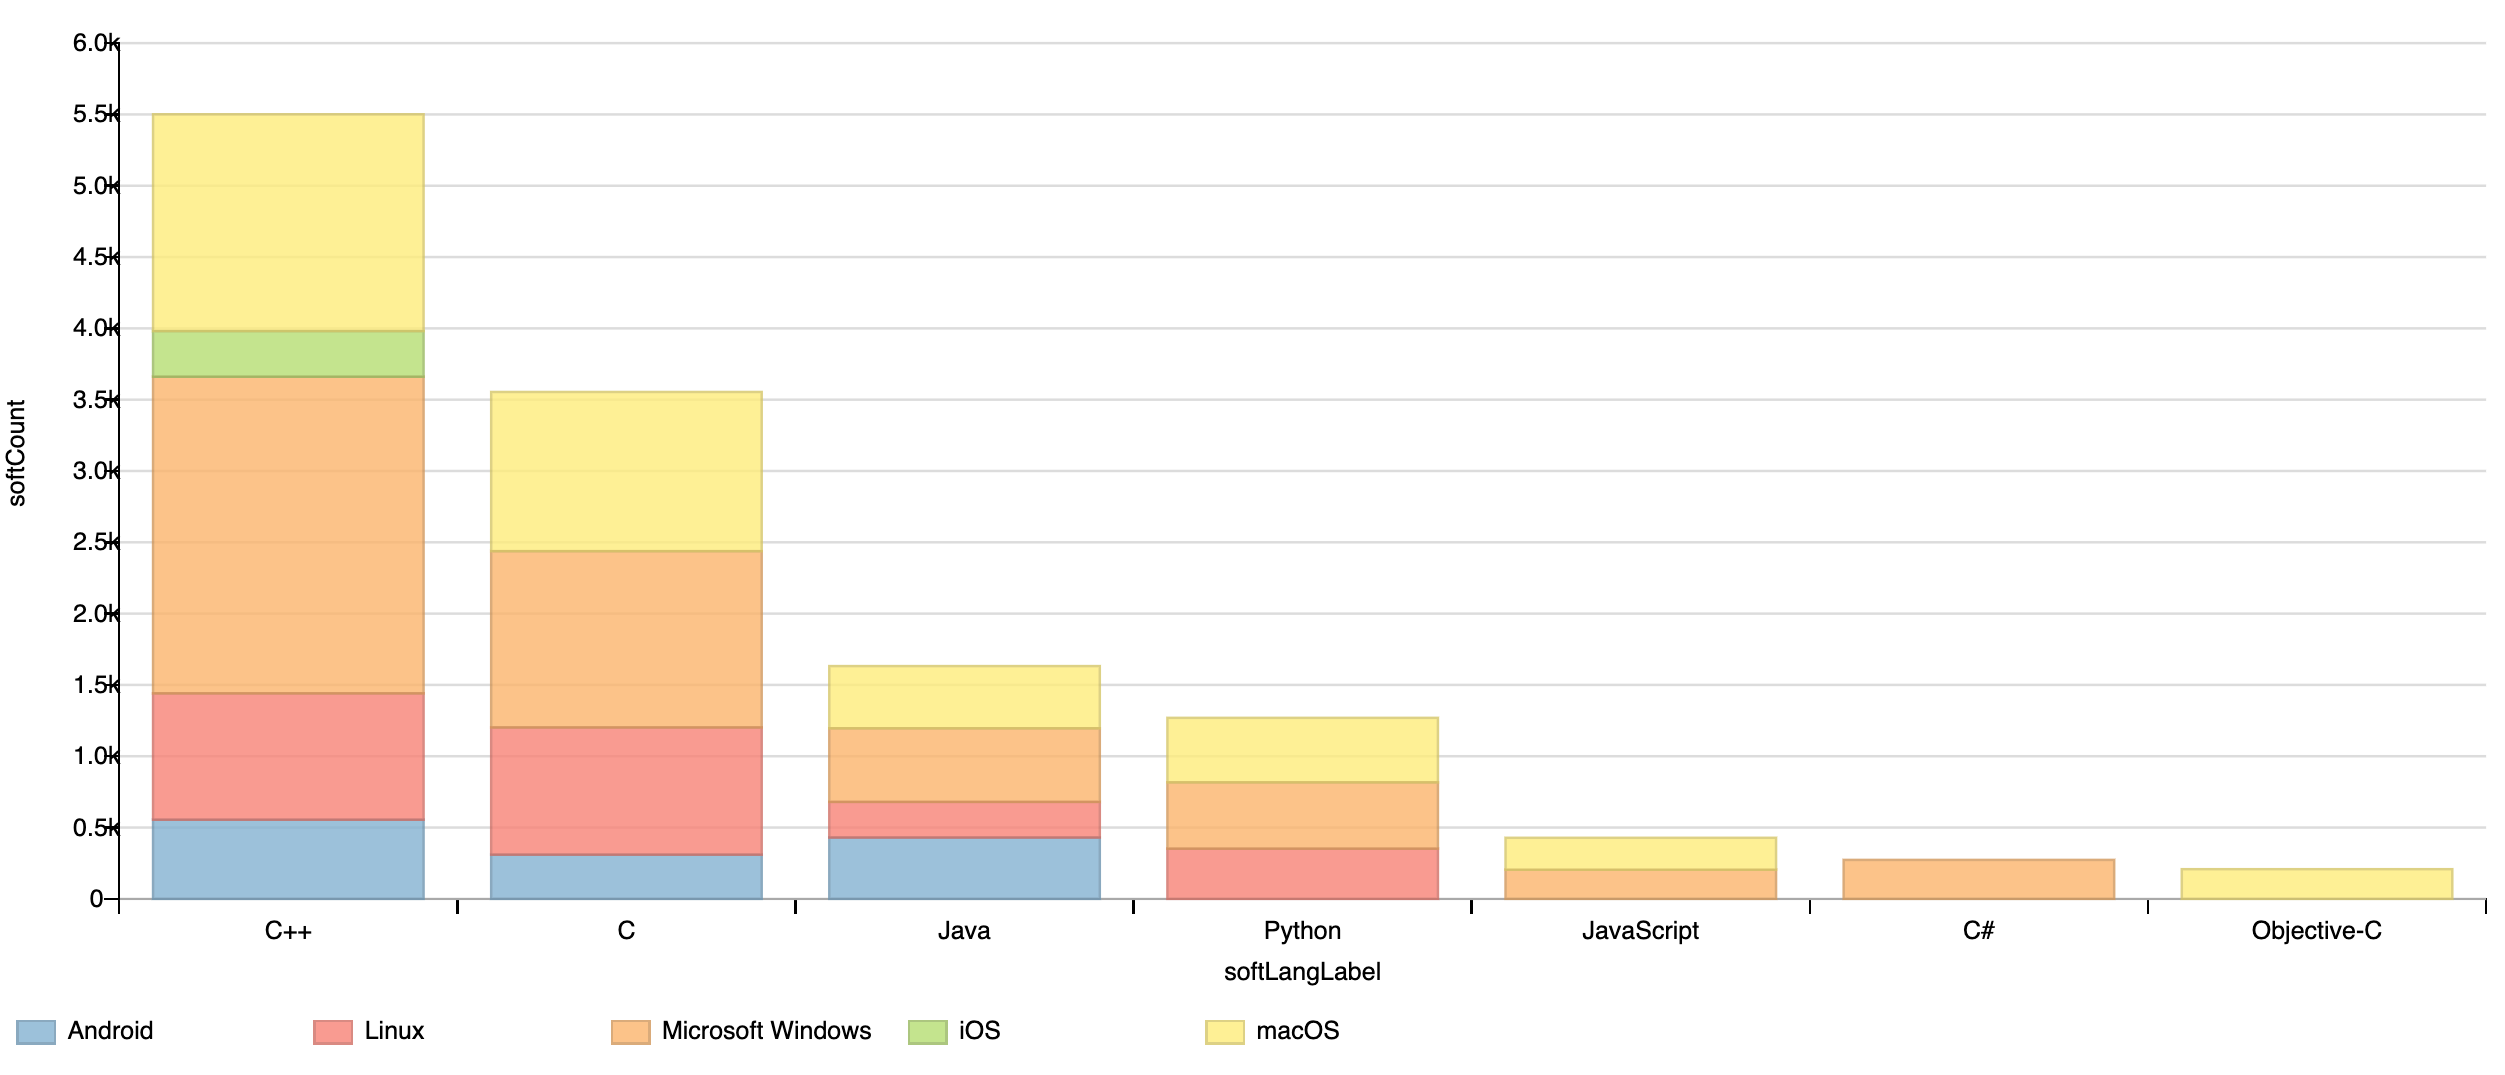
\includegraphics{./chapter/operating_system/Programming-languages-and-count-of-programms-written-on-them-and-OS-2020.png}
	\caption{Языки программирования и количества ОС, под которыми работают программы, написанные на них 2020 год.}
	\label{fig:count-software-written-on-languages}
\end{figure*}

Рассмотрим каждый из этих языков подробнее.

Большая часть программ на языке С++ пишется под windows (472 программы) и macOs (300 программ). Несмотря на то, что язык был разработан в 1972, он пока не теряет своей популярности за счет, вероятно, того, что используется для написания низкоуровневых приложений, т.к. по <<близости>> к аппаратному уровню уступает разве что ассемлеру.

Большая часть программ на языке С++ пишется под macOS (400 программ) и windows (700 программ) и Linux (400 программы). Вероятно, С++ будет лидировать еще долгое время, т.к. на текущий момент он используется для решений, требующих высокой производительности, чего не позволяют высокоуровневые языки, как Java или C\#.

Большая часть программ на языке Java пишется под macOS (196 программ) и Андроид (156 программ). Вероятно, Java пользуется популярностью за счет переносимости кода, т.е. код на Java запустится на любой машине с установленной JVM.

Большая часть программ на языке JavaScript пишется под macOS (100 программ) и Андроид (60 программ) и iOS (40 программ). Как правило, используется для написания клиентской части веб-приложений, что разработке сложных веб-приложений приводит к снижению нагрузки на сервер и увеличению скорости работы приложения.

Большая часть программ на языке Python пишется под macOS (212 программ) и Linux (107 программ). Высокоуровневый язык с низким порогом вхождения. Используется, например, для написания веб-приложений и анализа данных.

Глядя на гистограмму, можно сделать вывод, что каждый из данных языков занял свою <<нишу>> в области разработки ПО и применяется для определенного круга задач. Также вижно, что большая часть ПО пишется под macOS (900 программ), windows (1500 программ), Linux (1200 программ) или Андроид (300 программ).